\documentclass{standalone}
\usepackage[usenames,dvipsnames]{xcolor}
\usepackage{tikz}
\usetikzlibrary{arrows.meta}
\usetikzlibrary{decorations.pathreplacing}

\begin{document}

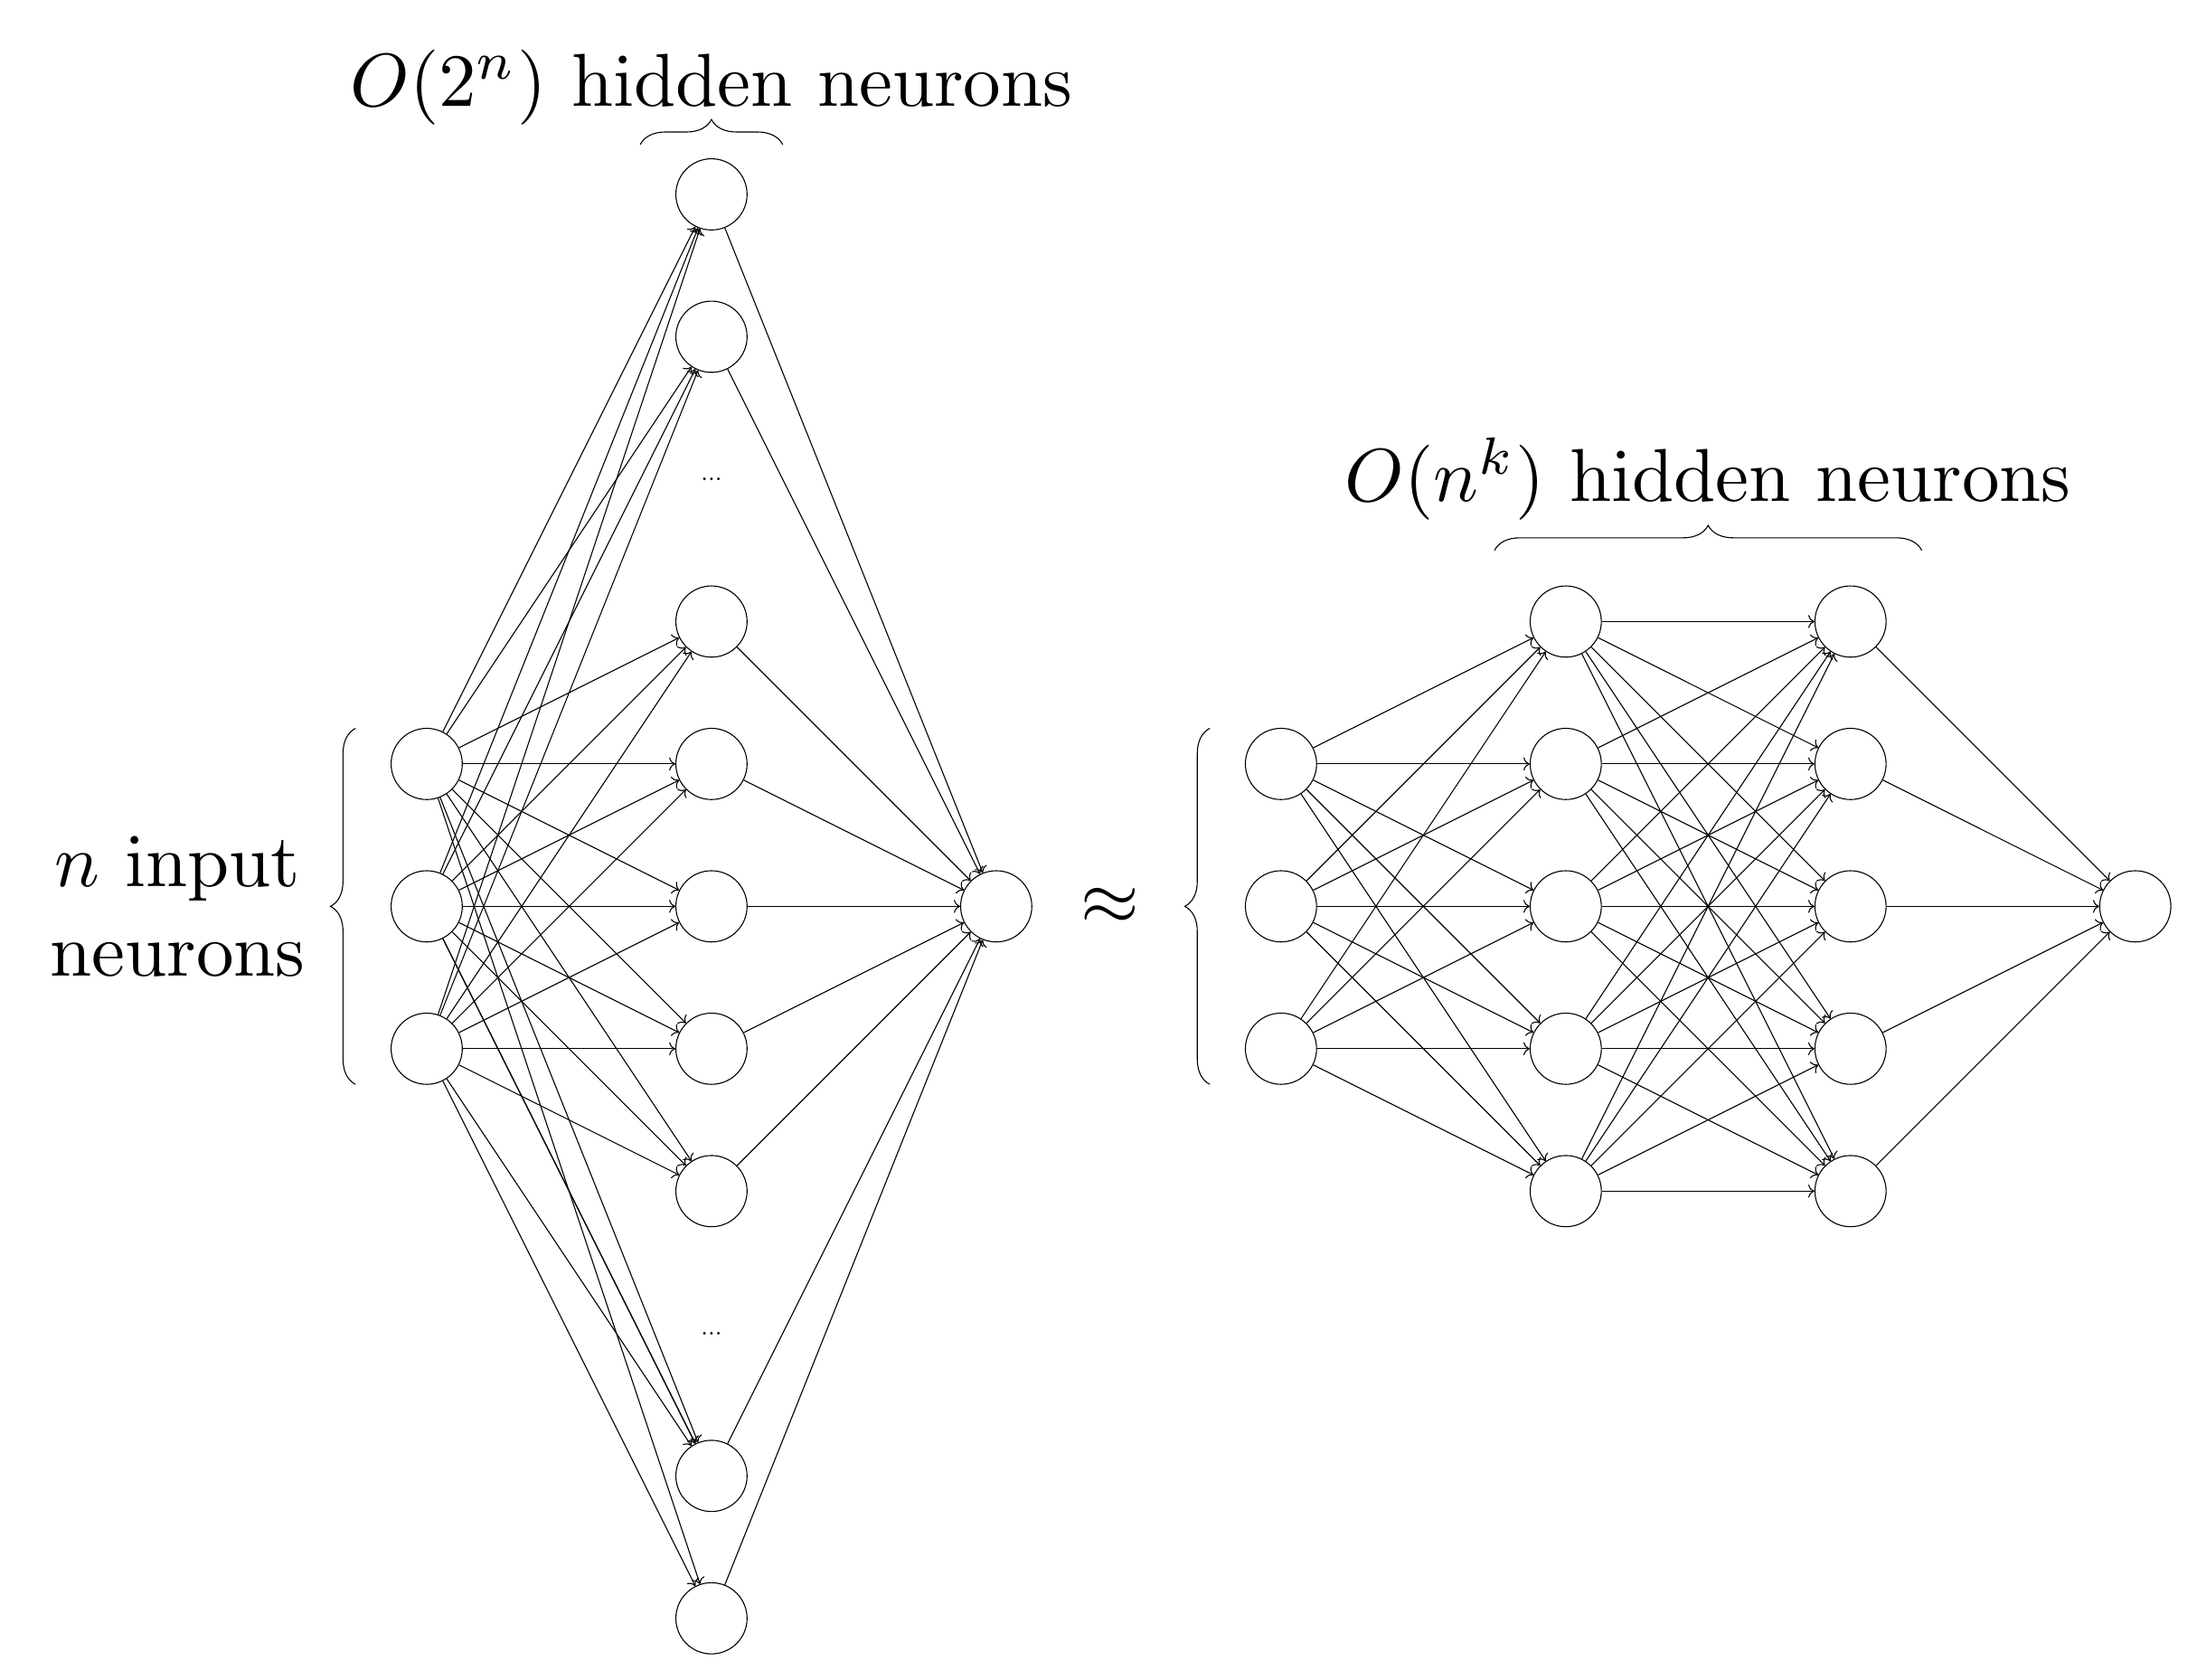
\begin{tikzpicture}

% SINGLE HIDDEN LAYER

% annotations

\draw [decorate, decoration={brace, amplitude=10pt}] (-1, -2.5) -- (-1,2.5);
\node[scale=3, align=center] at (-3.5,0) {$n$ input \\ neurons};

\draw [decorate,decoration={brace,amplitude=10pt}] (3,10.7) -- (5,10.7);
\node[scale=3] at (4,11.5) {$O(2^n)$ hidden neurons};


% input layer

\node[draw, circle, minimum size=1cm] (i1) at (0, 2) {};
\node[draw, circle, minimum size=1cm] (i2) at (0, 0) {};
\node[draw, circle, minimum size=1cm] (i3) at (0, -2) {};

% hidden layer
\node[draw, circle, minimum size=1cm] (h1) at (4, 10) {};
\node[draw, circle, minimum size=1cm] (h2) at (4, 8) {};
\node[] at (4, 6) {...};
\node[draw, circle, minimum size=1cm] (h3) at (4, 4) {};
\node[draw, circle, minimum size=1cm] (h4) at (4, 2) {};
\node[draw, circle, minimum size=1cm] (h5) at (4, 0) {};
\node[draw, circle, minimum size=1cm] (h6) at (4, -2) {};
\node[draw, circle, minimum size=1cm] (h7) at (4, -4) {};
\node[] at (4, -6) {...};
\node[draw, circle, minimum size=1cm] (h8) at (4, -8) {};
\node[draw, circle, minimum size=1cm] (h9) at (4, -10) {};

% output layer
\node[draw, circle, minimum size=1cm] (o1) at (8,0) {};

% input -> hidden
\draw [->] (i1) edge (h1) (i1) edge (h2) (i1) edge (h3);
\draw [->] (i2) edge (h1) (i2) edge (h2) (i2) edge (h3);
\draw [->] (i3) edge (h1) (i3) edge (h2) (i3) edge (h3);

\draw [->] (i1) edge (h4) (i1) edge (h5) (i1) edge (h6);
\draw [->] (i2) edge (h4) (i2) edge (h5) (i2) edge (h6);
\draw [->] (i3) edge (h4) (i3) edge (h5) (i3) edge (h6);

\draw [->] (i1) edge (h7) (i1) edge (h8) (i1) edge (h9);
\draw [->] (i2) edge (h7) (i2) edge (h8) (i2) edge (h8);
\draw [->] (i3) edge (h7) (i3) edge (h8) (i3) edge (h9);

% hidden -> output
\draw [->] (h1) edge (o1) (h2) edge (o1) (h3) edge (o1);
\draw [->] (h4) edge (o1) (h5) edge (o1) (h6) edge (o1);
\draw [->] (h7) edge (o1) (h8) edge (o1) (h9) edge (o1);



% TWO HIDDEN LAYERS

% annotations

\draw [decorate, decoration={brace, amplitude=10pt}] (11, -2.5) -- (11,2.5);
\node[scale=3, align=center] at (9.6,0) {$\approx$};

\draw [decorate,decoration={brace,amplitude=10pt}] (15,5) -- (21,5);
\node[scale=3] at (18,6) {$O(n^k)$ hidden neurons};


% input layer
\node[draw, circle, minimum size=1cm] (x1) at (12, 2) {};
\node[draw, circle, minimum size=1cm] (x2) at (12, 0) {};
\node[draw, circle, minimum size=1cm] (x3) at (12, -2) {};

% hidden layer 1
\node[draw, circle, minimum size=1cm] (y1) at (16, 4) {};
\node[draw, circle, minimum size=1cm] (y2) at (16, 2) {};
\node[draw, circle, minimum size=1cm] (y3) at (16, 0) {};
\node[draw, circle, minimum size=1cm] (y4) at (16, -2) {};
\node[draw, circle, minimum size=1cm] (y5) at (16, -4) {};

% hidden layer 2
\node[draw, circle, minimum size=1cm] (y6) at (20, 4) {};
\node[draw, circle, minimum size=1cm] (y7) at (20, 2) {};
\node[draw, circle, minimum size=1cm] (y8) at (20, 0) {};
\node[draw, circle, minimum size=1cm] (y9) at (20, -2) {};
\node[draw, circle, minimum size=1cm] (y10) at (20, -4) {};

% output layer
\node[draw, circle, minimum size=1cm] (z1) at (24,0) {};

% input -> hidden 1
\draw [->] (x1) edge (y1) (x1) edge (y2) (x1) edge (y3) (x1) edge (y4) (x1) edge (y5);
\draw [->] (x2) edge (y1) (x2) edge (y2) (x2) edge (y3) (x2) edge (y4) (x2) edge (y5);
\draw [->] (x3) edge (y1) (x3) edge (y2) (x3) edge (y3) (x3) edge (y4) (x3) edge (y5);

% hidden 1 -> hidden 2
\draw [->] (y1) edge (y6) (y1) edge (y7) (y1) edge (y8) (y1) edge (y9) (y1) edge (y10);
\draw [->] (y2) edge (y6) (y2) edge (y7) (y2) edge (y8) (y2) edge (y9) (y2) edge (y10);
\draw [->] (y3) edge (y6) (y3) edge (y7) (y3) edge (y8) (y3) edge (y9) (y3) edge (y10);
\draw [->] (y4) edge (y6) (y4) edge (y7) (y4) edge (y8) (y4) edge (y9) (y4) edge (y10);
\draw [->] (y5) edge (y6) (y5) edge (y7) (y5) edge (y8) (y5) edge (y9) (y5) edge (y10);

% hidden 2 -> output
\draw [->] (y6) edge (z1) (y7) edge (z1) (y8) edge (z1) (y9) edge (z1) (y10) edge (z1);

\end{tikzpicture}
\end{document}